\documentclass[11pt]{article}
\usepackage[backend=biber, style=numeric, url=true, doi=true]{biblatex}
\addbibresource{EFCM.bib}
\usepackage{url}
\usepackage{breakurl}
\usepackage[colorlinks=true, linkcolor=black, citecolor=blue, urlcolor=blue]{hyperref}
\usepackage{graphicx}
\graphicspath{{images/}}


\title{[Elements of Economics, Finance, and Computational Mathematics]}
\date{\today}
\author{Radu Briciu}
\begin{document}
\nocite{*}
\maketitle
\newpage
\begin{abstract}
	\noindent
	We examine an emerging pedagogical realm in which the importance of three major disciplines are considered in synchronicity. The aim is to understand the coherence of an interdisciplinary science formed around modern Economics, Finance, and Computational Mathematics. We recognize the rapidly evolving progress in data encoding techniques and contemplate economic, financial, and societal phenomena that may arise from technology evolving at increasing rates.
\end{abstract}
\vspace{5em}
Join the discord: https://discord.gg/HHStaC4h\\
Join the subreddit: https://www.reddit.com/r/MaryleboneResearch/


\newpage
\tableofcontents	
\newpage

\section{Introduction}
I am developing this paper on my own in the hopes it becomes a larger group project. I believe all learning is a collective matter and cordially invite all people interested into the discussion of such a portfolio of ideas.

\section{Recent computational developments}
\subsection{Zero Knowledge Proofs}
Zero Knowledge proofs~\cite{ernstberger_2024_do} are a familiar cryptographic concept with recent applicability to scaling financial circuitries~\cite{leethorp_2022_fnet}.
\subsection{Machine learning in numerical methods}
Machine learning methods allow for greater accuracy in all manner of numerical computation and model interpretation tasks. Interpretability of models allows for easier and more accurate volatility modelling~\cite{beck_2019_machine}~\cite{kirenz_2022_using}~\cite{parr_2021_partial}~\cite{yuan_2024_deep}.

\subsection{Artificial General Intelligence (AGI)}
\subsubsection{OpenAI}
\subsubsection{Google}
\subsubsection{GitHub}

\section{Internet tools}
With technological hardware becoming increasingly accessible, powerful internet tools emerge that may require immediate attention or regulation. Others however, are useful in pedagogical applications.
\subsection{Kleros~\cite{zhuk_2023_applying}}
Kleros~\cite{zhuk_2023_applying} aims to automate certain commercial mediation processes by use of blockchain technology allowing for financial arbitrage in conflict resolution scenarios.
\subsection{Tornado Cash~\cite{nadler_2023_tornado}~\cite{pertsev_2019_tornado}}
Tornado Cash is a peculiar blockchain smart contract protocol that allows users to send and receive cryptocurrency payments completely anonymously. The protocol has purportedly been flagged by US authorities leading to very little utilization.
\subsection{Cofence~\cite{cofense_2024_phishme}}
Cofence present a cybersecurity email protection algorithm with integrated human vetting.
\subsection{Polymarket~\cite{polymarket}}
Polymarkets are an interesting phenomenon that, with sufficient volume, may have significant economic effects on an observed event.
\subsection{Quantgov~\cite{quantgovhome_2025_quantgov}}
Quantgov seemingly publicises various regulatory documents potentially in the idea to cut red tape.
\subsection{TinyURL~\cite{a2019_tinyurlcom}}
TinyURL advertises a useful link shortening tool with added security features along a paid subscription. Modern cryptographic links are long and may seem intimidating especially when domain names change rapidly.
\subsection{MyBib~\cite{mybib_2018_mybib}}
MyBib is a powerful tool for understanding how BibTeX files work, bringing new dimensions to independent research.
\subsection{ORCiD~\cite{orcid_2019_orcid}}
ORCiD provides an easy way for researchers to connect and share work with cutting edge technology at their fingertips.
\subsection{ProtonMail~\cite{kobeissi_2018_an}}
ProtonMail is a popular emailing service based in Switzerland claiming to offer end-to-end encryption. The existence of such services call into question the feasibility of further scaling to internet privacy infrastructure. An analysis~\cite{kobeissi_2018_an} on the service's security is offered by Kobeissi.
\subsection{The Wikimedia Foundation~\cite{a2018_wikimedia}}
The Wikimedia Foundation emerged as a financial supporter of the Wikipedia project, allowing independent researchers to support the movement around freedom of scientific information.
\subsection{Data Annotation~\cite{data}}
Data Annotation is a website that purportedly pays its users to redact and assess AI chatbot prompts and responses.
\subsection{Online Museums}
Berkeley, University of California publishes art photography online~\cite{a2024_library} for universal visual access to painting, scriptures, documents, sculptures, trinkets, and other art history relics.
\subsection{Subdial~\cite{a2023_subdial}}
Subdial is an online marketplace where watches are verified per the listing specification.
\subsection{Pentester~\cite{a2024_pentester}}
Pentester is a peculiar website that supposedly attempts to collect the digital footprint left behind by an input email address.
\subsection{EconViz~\cite{econvizorgmacroeconomicvisualizations_2025_econvizorg}}
EconViz is a free online tool that helps visualize classical economic theory.

\section{\textit{The OS wars}}
\subsection{Environment Intractability}
\subsubsection{Entropy Pooling~\cite{vorobets_2024_portfolio}}
\subsubsection{Stochastic Volatility~\cite{heston_1993_a}~\cite{briciu_2024_estimating}}
\section{Quantitative trading strategies}
\subsection{Macroeconomic trend prediction using live shipping data}
\subsection{Political spectrum matrix sentiment analysis}
\begin{figure}[h!]
	\centering
	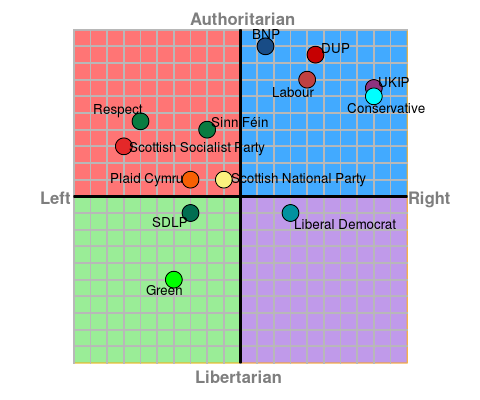
\includegraphics[width=0.8\textwidth]{uk2010.png}
	\caption{UK Political Spectrum}
	\label{fig:UKCompass}
\end{figure}
\newpage
\section{Blockchain security and pipeline transparency}
\subsection{Commodities markets}
\subsection{FX option markets}
\subsection{Commerical legal services}

\section{Engineering concepts}
\subsection{Integrating solar panels into protected forestry domain}

\newpage
\printbibliography
\addcontentsline{toc}{section}{References}
\end{document}